\chapter{Estrutura do documento}
A estrutura se refere à divisão de um documento em partes, capítulos, seções e níveis adicionais de estrutura.
\begin{figure}[h]
    \centering
    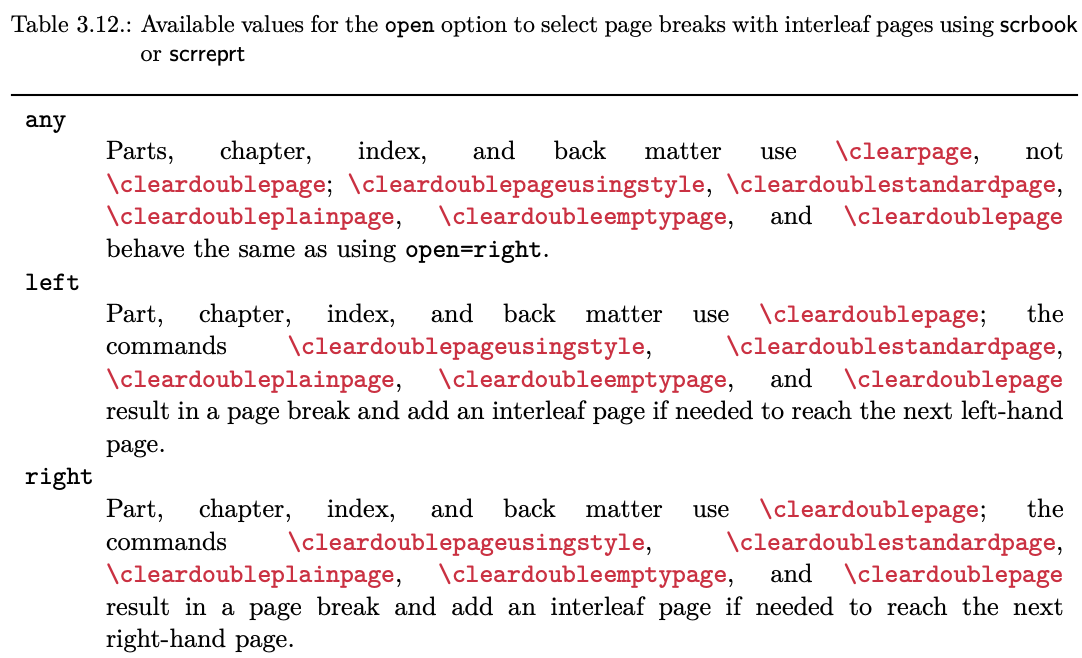
\includegraphics[width=0.80\linewidth]{imagem17.png}
    %\caption{Enter Caption}
    \label{fig:3_12}
\end{figure}

\minisec{open=method}
As classes \KOMAScript\ \texttt{scrbook} e \texttt{scrreprt} oferecem a você a opção de onde começar um novo capítulo com impressão frente e verso. Por padrão, \texttt{scrreprt} inicia um novo capítulo na próxima página. Isso é equivalente ao método any. No entanto, \texttt{scrbook} inicia novos capítulos na próxima página à direita. Isso é equivalente ao método right e geralmente é usado em livros. Mas às vezes os capítulos devem começar na página esquerda de uma página dupla. Você pode fazer isso com o método left. Você pode encontrar um resumo dos valores disponíveis na tabela 3.12. A tabela também descreve os efeitos de \char`\\\texttt{clear\-dou\-ble\-pa\-ge}, \char`\\\texttt{clear\-dou\-ble\-pa\-ge\-u\-sing\-sty\-le}, \char`\\\texttt{clear\-dou\-ble\-stan\-dard\-pa\-ge}, \char`\\\texttt{clear\-dou\-ble\-plain\-pa\-ge} e \char`\\\texttt{clear\-dou\-ble\-empty\-pa\-ge} (consulte a seção 3.13, página 87).

Como o \LaTeX\ não diferencia entre páginas esquerdas e direitas na impressão de um lado, a opção não tem efeito nesse caso.

Na classe \texttt{scrartcl}, a seção é o primeiro elemento estrutural abaixo da peça. Por esse motivo, \texttt{scrartcl} não suporta essa opção.

\begin{figure}
    \centering
    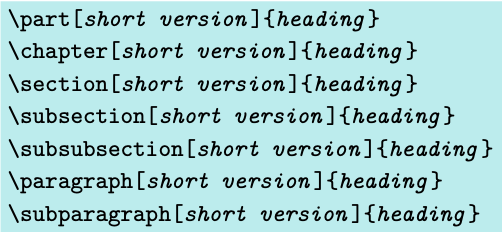
\includegraphics[width=0.65\linewidth]{imagem18.png}
    \label{fig:img18}
\end{figure}

Os comandos de seccionamento padrão no \KOMAScript\ funcionam da mesma forma que aqueles nas classes padrão. Assim, você pode especificar um texto alternativo para o índice e títulos como um argumento opcional para os comandos de seccionamento.

No entanto, com a opção \texttt{headings=optiontohead}, o \KOMAScript\ usa apenas a versão curta do argumento opcional no título, não no índice. Claro, esse texto só aparecerá se você usar um estilo de página que coloque o nível de seccionamento correspondente no título. Veja a seção 3.12 e o capítulo 5. Com a opção \texttt{headings=optiontotoc}, o \KOMAScript\ usa a versão curta (\textit{short version}) do argumento opcional exclusivamente para o índice e não para o título. No entanto, a entrada será mostrada apenas se o \texttt{tocdepth counter} for grande o suficiente (veja a seção 3.9, página 76). Com a opção \texttt{headings=optiontoheadandtoc}, o \KOMAScript\ usa a versão curta do argumento opcional tanto no índice quanto no título. Todas essas três opções ativam a interpretação estendida da versão curta do argumento opcional, que não está ativa por padrão.

A interpretação estendida do argumento opcional verifica se há um sinal de igual na versão curta. Se houver, o argumento opcional será interpretado como uma lista de opções. Quatro opções
\begin{itemize}
    \item \texttt{head=running head},
    \item \texttt{tocentry=table of contents entry},
    \item \texttt{reference=reference title} e 
    \item \texttt{nonumber=simple switch}
\end{itemize}

são suportadas com este formato. Para usar vírgulas ou sinais de igual dentro dos valores dessas opções, você deve colocá-los entre chaves.

Observe que este mecanismo só funciona enquanto o \KOMAScript\ controlar os comandos de seccionamento. Se você usar um pacote que redefine os comandos de seccionamento do \KOMAScript\ ou do kernel interno do \LaTeX, o \KOMAScript\ não poderá mais fornecer este mecanismo estendido. Isso também se aplica a uma extensão do \KOMAScript\ que está sempre ativa: comandos de seccionamento sem texto de título não criam entradas no índice. Se você realmente quiser uma entrada com texto de título vazio, você pode usar uma entrada invisível como \mbox{}.

\textbf{Exemplo}: Suponha que você tenha um documento com títulos de capítulo muito longos. Esses títulos devem aparecer no índice, mas você quer limitar o título corrente a títulos curtos de uma única linha. Você pode fazer isso com o argumento opcional de \char`\\\texttt{chap\-ter}.

\begin{figure}[h]
    \centering
    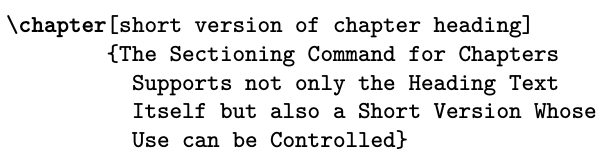
\includegraphics[width=0.60\linewidth]{imagem14.png}
    \label{fig:img14}
\end{figure}



